\documentclass[titlepage,12pt,a4paper]{article}
\usepackage[a4paper]{geometry}
\usepackage{amsmath}
\usepackage{amssymb}
\usepackage{enumitem}
\usepackage{commath}
\usepackage{mathtools}
\usepackage{graphicx}
\usepackage{dirtytalk}
\usepackage{csquotes}
\usepackage{hyperref}
\usepackage{tabto}
\usepackage{gensymb}
\usepackage{graphicx}
\usepackage{listings}
\usepackage{sidecap}
\usepackage{wrapfig}
\usepackage{pdfpages}
\usepackage[toc,page]{appendix}
\usepackage{filecontents}
\usepackage{lipsum}

\bibliographystyle{IEEEtran}

\usepackage{color}
\definecolor{dkgreen}{rgb}{0,0.6,0}
\definecolor{gray}{rgb}{0.5,0.5,0.5}
\definecolor{mauve}{rgb}{0.58,0,0.82}

\lstset{frame=tb,
  language=C++,
  aboveskip=3mm,
  belowskip=3mm,
  showstringspaces=false,
  columns=flexible,
  basicstyle={\small\ttfamily},
  numbers=left,
  numberstyle=\footnotesize,
  stepnumber=1,
  numbersep=5pt,
  keywordstyle=\color{blue},
  commentstyle=\color{dkgreen},
  stringstyle=\color{mauve},
  breaklines=true,
  breakatwhitespace=true,
  tabsize=3
}

\usepackage{fancyhdr}
\setlength{\headheight}{15.2pt}
\pagestyle{fancy}
\fancyhf{}
\lhead{ \fancyplain{}{COMP3431: Robotic Software Architecture} }
\rfoot{ \fancyplain{}{\thepage} }


\begin{document}
\begin{titlepage}
    \begin{center}
        \vspace*{3cm}
        
        \Huge
        \textbf{COMP3431\\}
        \title{}
        \vspace{0.5cm}
        \Huge
        \textbf{Robotic Software Architecture}
        
        \vspace{0.54cm}
        
        \Large
        Assignment 2: Report
        
        \vspace{5cm}

	\normalsize
	Aaron Ramshaw\\
	Simon Robilliard\\
    Lucy Kidd\\
	Wayne Yeung
        
	\vfill
        
        \Large
        November 3, 2015
        
    \end{center}
\end{titlepage}

\pagebreak

\section{Introduction}
The Mini Emu is part of the rescue challenge, with the aim of our project being to develop the robot to navigate through a course, with the robot operator controlling it from an external computer.\\

\noindent The project required the development of an interface between a Raspberry Pi v2, Dynamixel motors and a Raspberry Pi Camera Module to form a mini EMU Robot. Software would be developed using Robot Operating System (ROS) such that the EMU could be controlled remotely using a Logitech gamepad controller and an image stream. The mini EMU consists of a rectangular chassis with four wheels connected. A long arm is mounted, via a motor to the upper carriage of the chassis, and two motors atop the arm create two more pivot points, with the top motor holding the Raspberry Pi Camera. An already constructed mini EMU can be seen in Figure \ref{fig:emu}.

\section{Background}
Robot Operating System (ROS) is an open-source robotics platorm. It provides a range of useful services including: ‘hardware abstraction, low-level device control, implementation of commonly-used functionality, message-passing between processes, and package management’ [1]. Within the ROS community there are open-source packages available for a range of sensors and drivers, this includes the Raspberry Pi camera and Dynamixel Motors. ROS also provides tools to run code across multiple computers at once, hence provides the perfect software foundations for this project.\\

\noindent The Raspberry Pi is advertised as a ‘credit card sized computer’ which can be plugged into a display via a High-Definition Multimedia Interface (HDMI) cable and uses a standard USB keyboard and mouse. The tiny computer consists of a 900 MHz quad–core Central Processing Unit, a 1GB Synchronous Dynamic Random-Access Memory (SDRAM) and OS of user choice that is stored on a microSD card. There are 30 plus General Purpose Input – Output (GPIO) pins, four USB inputs and a 30 way camera connector, which makes the Raspberry Pi perfect for robotics applications.\\

\noindent The Dynamixel AX-12A servo actuator from the Korean manufacturing company Robitis, has the ability to track it's own speed, temperature, shaft position, voltage and load. The shaft position of of the ax-12 actuator can be adjusted individually for each motor, allowing a different speed and strength for each motor [2]. Each motor can be initialised as either a standard servo motor or as a continuous rotation servo, hence the motor is applicable for use as the EMU robots’ wheel drivers and arm pivot points.\\

\noindent The Raspberry Pi Camera Module is a small camera that connects to a Raspberry Pi via a 30 way ribbon cable. The Raspbian OS has built in drivers for cameras connected via this connector, and an Open-Source Application Program Interface (API) for C++ available for use [3].  The camera has video modes of up to 1080p at 30 frames per second (fps) and a still frame resolution of up to 5 Megapixels, hence provides potential for a high quality video stream.\\

\newpage
\section{Chassis and Hardware}
The Mini Emu robot was designed by the Intelligent Robots Group at the Department of Computing, Curtin University. We have 3D printed two robots for use, both equipped with Raspberry Pi and camera. The robots have 4 Dynamixel motors for the wheels, and 3 Dynamixel motors for the arm.\\

\begin{figure}
  \centering
      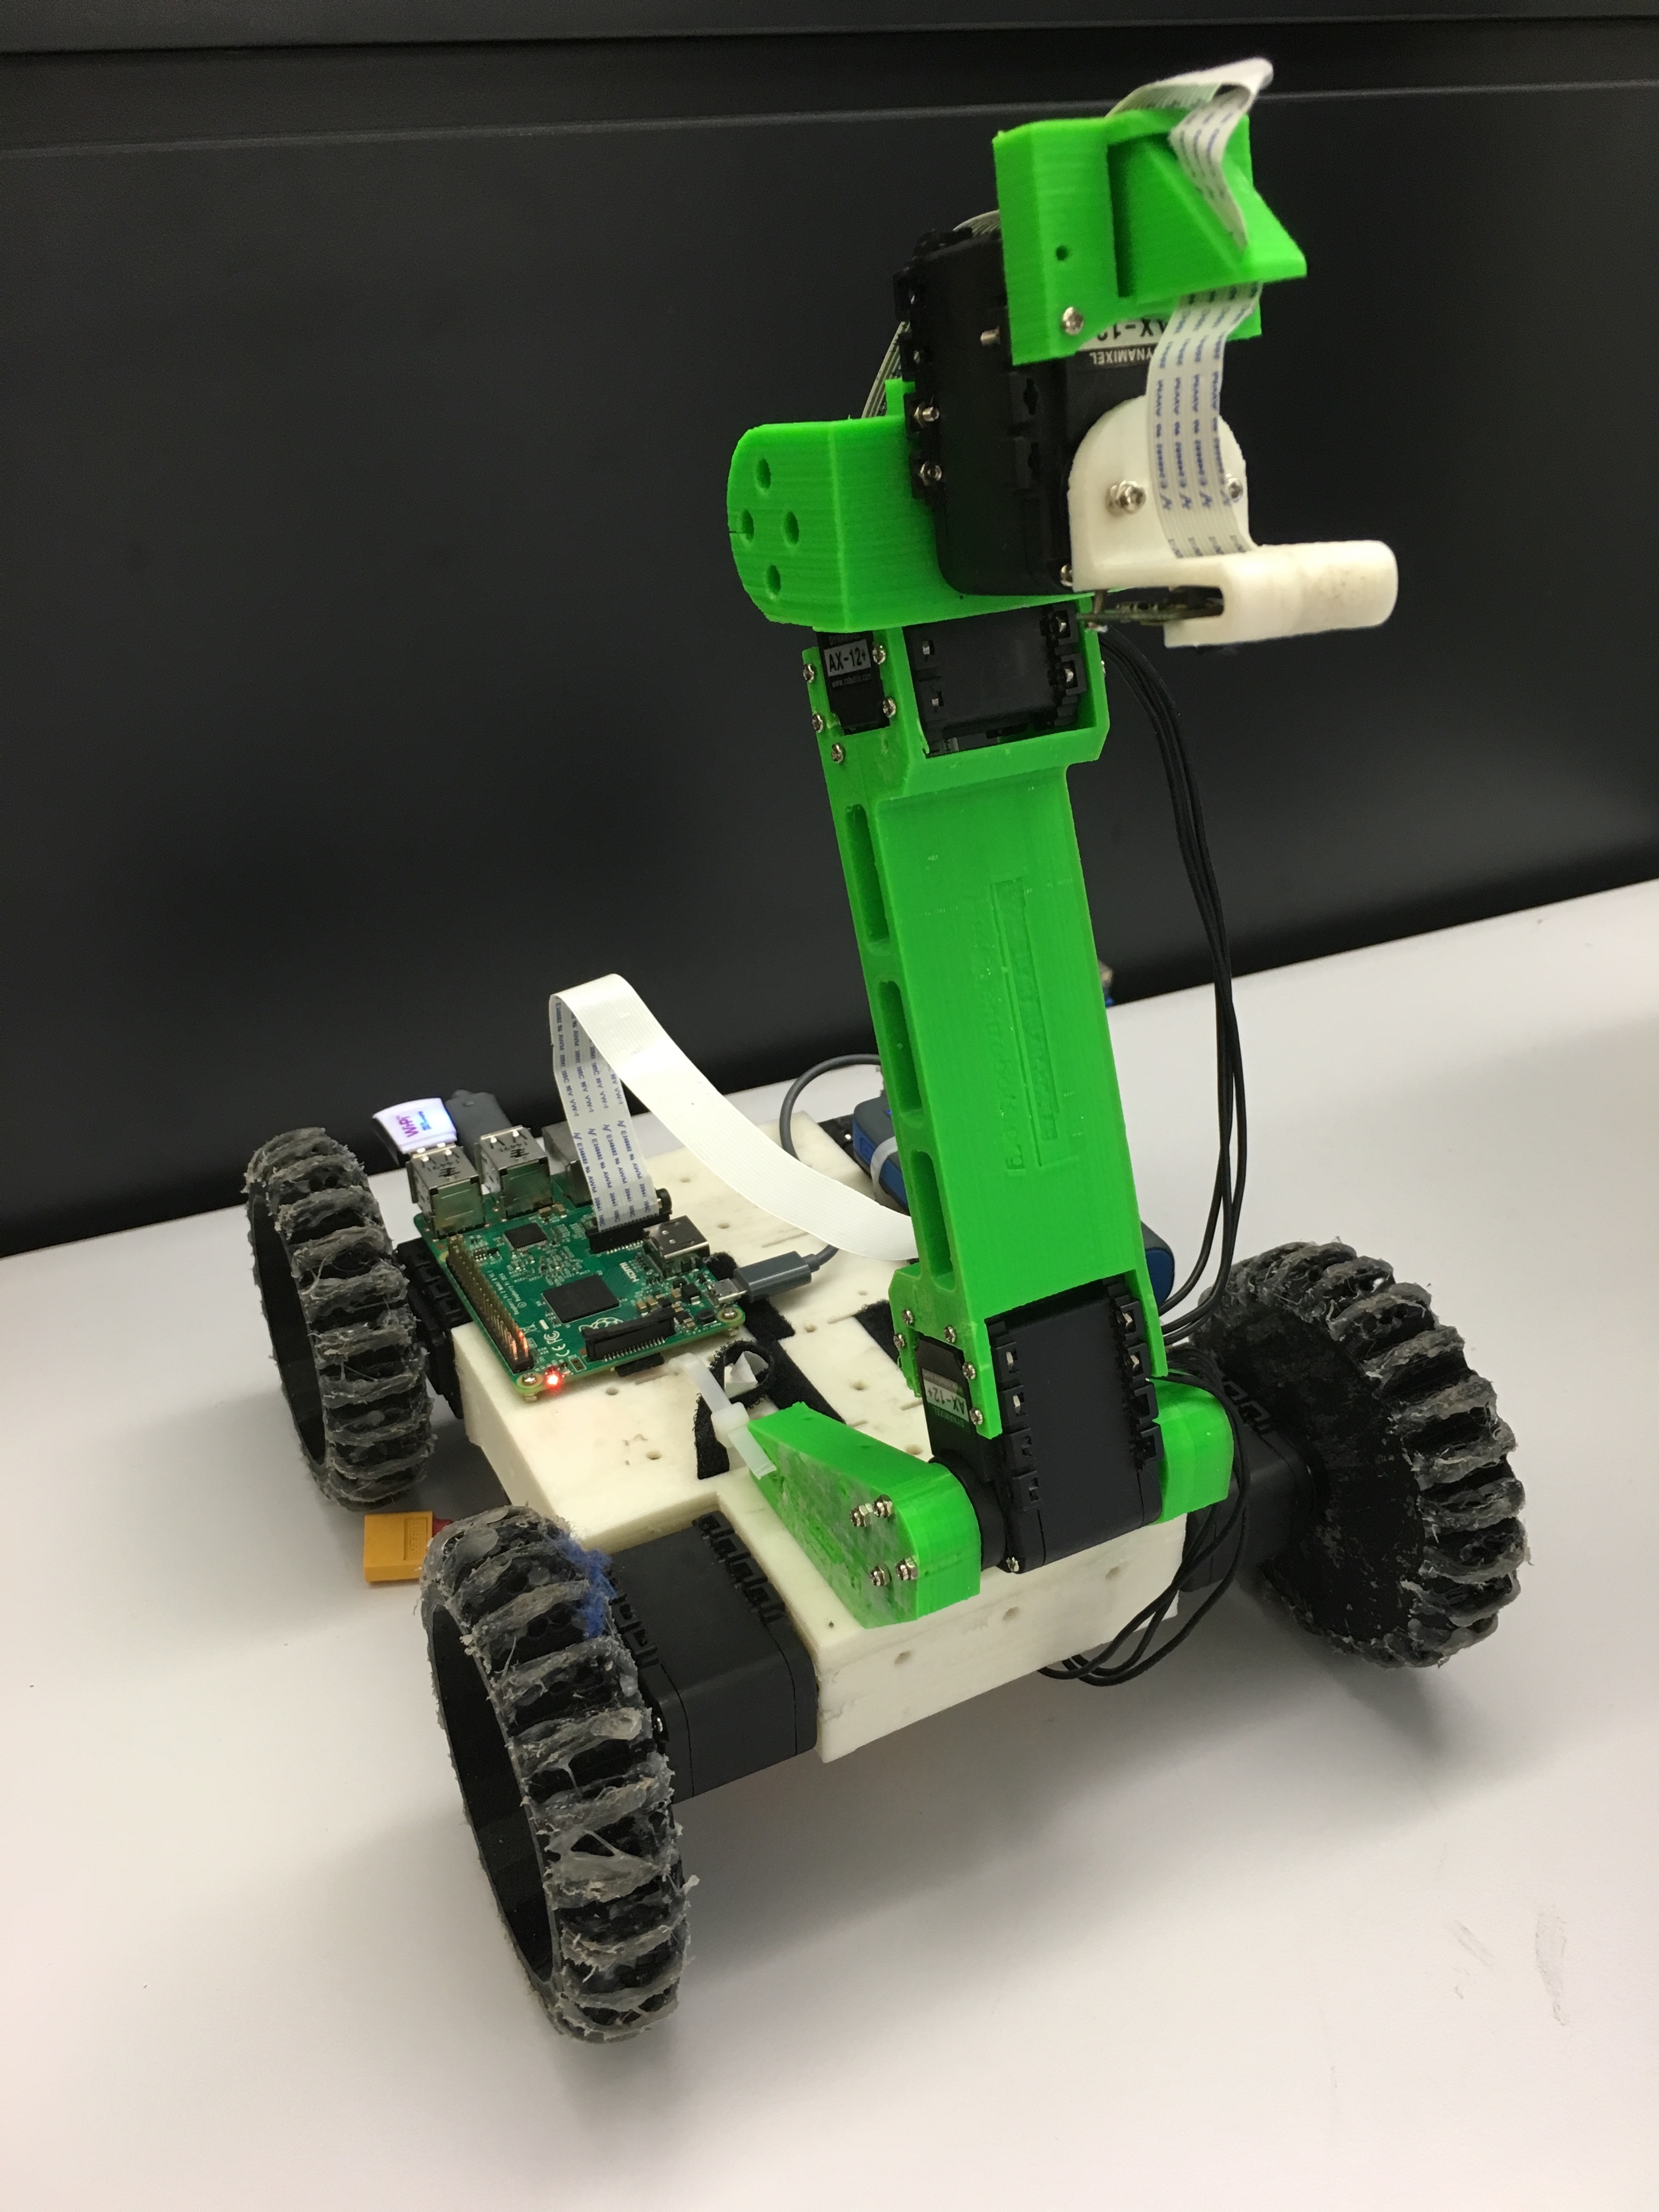
\includegraphics[height=300pt]{robot}
  \caption{Mini Emu Robot}
  \label{fig:emu}
\end{figure}


\noindent A detachable cardboard underside cover is used to hold in the cables and prevent the components catching or hitting the course.

\newpage
\section{Software}
\subsection{Architecture}
Debian based Raspbian is the official supported operating system for the Raspberry Pi. The OS is installed to the microSD card of the Pi. Raspbian was chosen because of it’s ease of installation and full support and compatibility with the Pi. ROS Indigo is the software platform used for the robot. Appendix A shows the ROS node graph of the project.


\subsection{Dependencies}

\noindent The project makes use of the Dynamixel Controllers package - the low level drivers for the Dynamixel motors. The Joystick Drivers package is used to receive commands from the Logitech controller. In addition, Raspicam drivers are used to interface with the Raspberry Pi camera.
The four nodes in our package are Commander, Emu State Publisher, Image Publisher and Joystick Converter.\\

\noindent Due to the ARM architecture and OS used on the Raspberry Pi, most of these packages are not available pre-built. Instead, \texttt{rosinstall\_generator}, should be used to download all required dependencies, and then \texttt{catkin\_make\_isolated} to compile into the \texttt{/opt/ros/indigo/} directory.

\subsection{Motor Configuration}
To control and track the motion and position of the seven motors across the mini EMU robot, the \texttt{dynamixel\_motor} [4] ROS package was used. This ROS package provides drivers for the dynamixel motors, and exposes control and tracking of the motors through ros topics that can be published and subscribed to. \\

\noindent The \texttt{dynamixel\_motor} package works by setting up a named controller for each motor in the robot. To initialise these controllers, two files are required. The first is a \texttt{motor.yaml} file which specifies:
\begin{itemize}
    \item The id of the motor to be controlled
    \item The type of controller required (either torque or position)
    \item The name of the controller, which will then be used as the name of the topic used to control and track the motor.
\end{itemize}
Below is an example of how a wheel motor would be configured.

\begin{lstlisting}
pan_controller_1:
    controller:
        package: dynamixel_controllers
        module: joint_torque_controller
        type: JointTorqueController
    joint_name: pan_joint_1
    joint_speed: 1.17
    motor:
        id: 7
        init: 512
        min: 0
        max: 4095
\end{lstlisting}


\noindent The second file is a motor spawner launch file, that launches a \texttt{controller\_spawner} for each of the controllers named in the motor.yaml file. The controller spawner generates a dynamixel controller for the motor. Below is an example of how a motor controller would be launched for the motor named \texttt{pan\_controller\_1}\\

\begin{lstlisting}
<node name="pan_gcontroller_spawner" pkg="dynamixel_controllers" type="controller_spawner.py"
        args="--manager=dxl_gmanager
              --port pan_gtilt_port
              pan_controller_1"
        output="screen"/>
\end{lstlisting}


\noindent This will then generate two ROS topics, \texttt{pan\_controller\_1/command} and\\ \noindent\texttt{pan\_controller\_1/state}. The first is a topic that can be published to with a motor speed or position, depending on whether the motor is in wheel mode or in position mode. The second is a topic that can be subscribed to that publishes information about the motor speed and position.

\newpage
\subsection{Commander}
This node is responsible for subscribing to the the topics published by Joystick Converter for controller input and motor state from Emu State Publisher. It then publishes appropriate commands to the 7 motor controllers.\\

\noindent The four wheel motors are set to pan mode which allows us to specify speeds, published to topics \texttt{/pan\_controller\_[1-4]/command} which take type \texttt{Float64} messages. The three arm motors are set to servo tilt mode which allows us to specify an angle, published to topics \texttt{/tilt\_controller\_[1-3]/command}, which also take type \texttt{Float64} messages (angle in radians).\\

\noindent The \texttt{joy\_stick\_converter} node publishes to two topics \texttt{motor\_command\_vector} and \texttt{servo\_command\_vector}. These two topics are \texttt{TwistStamped} messages, containing 2 3D vectors \texttt{linear} and \texttt{angular}.\\

\noindent For \texttt{motor\_command\_vector} we are only concerned with the \texttt{x} and \texttt{y} values of the \texttt{twist.linear} vector. This is the direction vector for the movement of the robot. We split up the components into left and right movement, then publish the speed \texttt{Float64} value to the left and right side motors respectively. These four motors controlling the wheels are set to pan mode, which allows us define a speed to run at.\\

\noindent Similarly, the node listens to \texttt{servo\_command\_vector}, which gives directions regarding the movement of the 3 motors making up the arm. Here we consider both the \texttt{twist.linear} and \texttt{twist.angular} vectors. The values of the linear vector are used to increment the position of the arm (all 3 \texttt{x}, \texttt{y} and \texttt{z} for the 3 motors) by publishing new incremented positions to \texttt{/tilt\_controller\_[1-3]/command} after reading the current positions from \texttt{/servo\_controller\_[1-3]/state}. The \texttt{twist.angular} vector is read to set the arm motors into set default positions. Instead the given angles are simply published to the \texttt{/tilt\_controller\_[1-3]/command} topics. \\

\noindent Due to the physical constraints of the chassis, limits are set on the arm motor angles to prevent pushing on the frame and pulling on cables. These limits are taken from ROS parameters at launch and override the \texttt{/tilt\_controller\_[1-3]/command} values when appropriate. The middle joint motor is also programmatically limited when the arm is extended past the base at an angle greater than 90 degrees - a position which uses the arm to push the whole robot chassis up. This retracts the camera joint, preventing the more fragile camera module from being damaged.\\

\noindent In addition, to facilitate easy and natural movement from the perspective of the robot driver (using the camera stream), the middle motor is calibrated with the arm base motor such that vertical camera angle remains constant when the arm base motor is moved. This is done by moving the middle joint motor in the opposite direction to the base joint.\\

\subsection{Emu State Publisher}
This node subscribes to the topics \texttt{/tilt\_controller\_[1-3]/state} which give the current positions of the three arm servo motors. It collates the data from the motors and publishes messages of type \texttt{JointState} to topic \texttt{/joint\_states}. This is part of the robot model visualisation, the ROS \texttt{robot\_state\_publisher} takes the \texttt{/joint\_states} topic and calculates the appropriate transforms, published to the \texttt{/tf} topic. RViz can then take the transforms, along with the URDF and model the position of the arm as it moves. \\

\subsection{Image Publisher}
This node interfaces with the Raspberry Pi camera through the Raspicam drivers (not a ROS package) and publishes messages of type \texttt{sensor\_msgs::Image} to the topic \texttt{/camera\_image}.\\

\noindent The node takes settings defined in the launch file from the parameters server which define image resolution, and whether video stabilisation is turned on. These settings are defined dynamically to allow optimisations based on network speed.\\

\noindent In addition, the \texttt{republish} node in the ROS \texttt{image\_transport} package is then used, subscribing to the \texttt{/camera\_image} node, then compressing the image out to \texttt{/camera\_repub}. This significantly increases the framerate on the robot driver's viewing computer.

\newpage
\subsection{Joystick Converter}

\begin{figure}
  \centering
      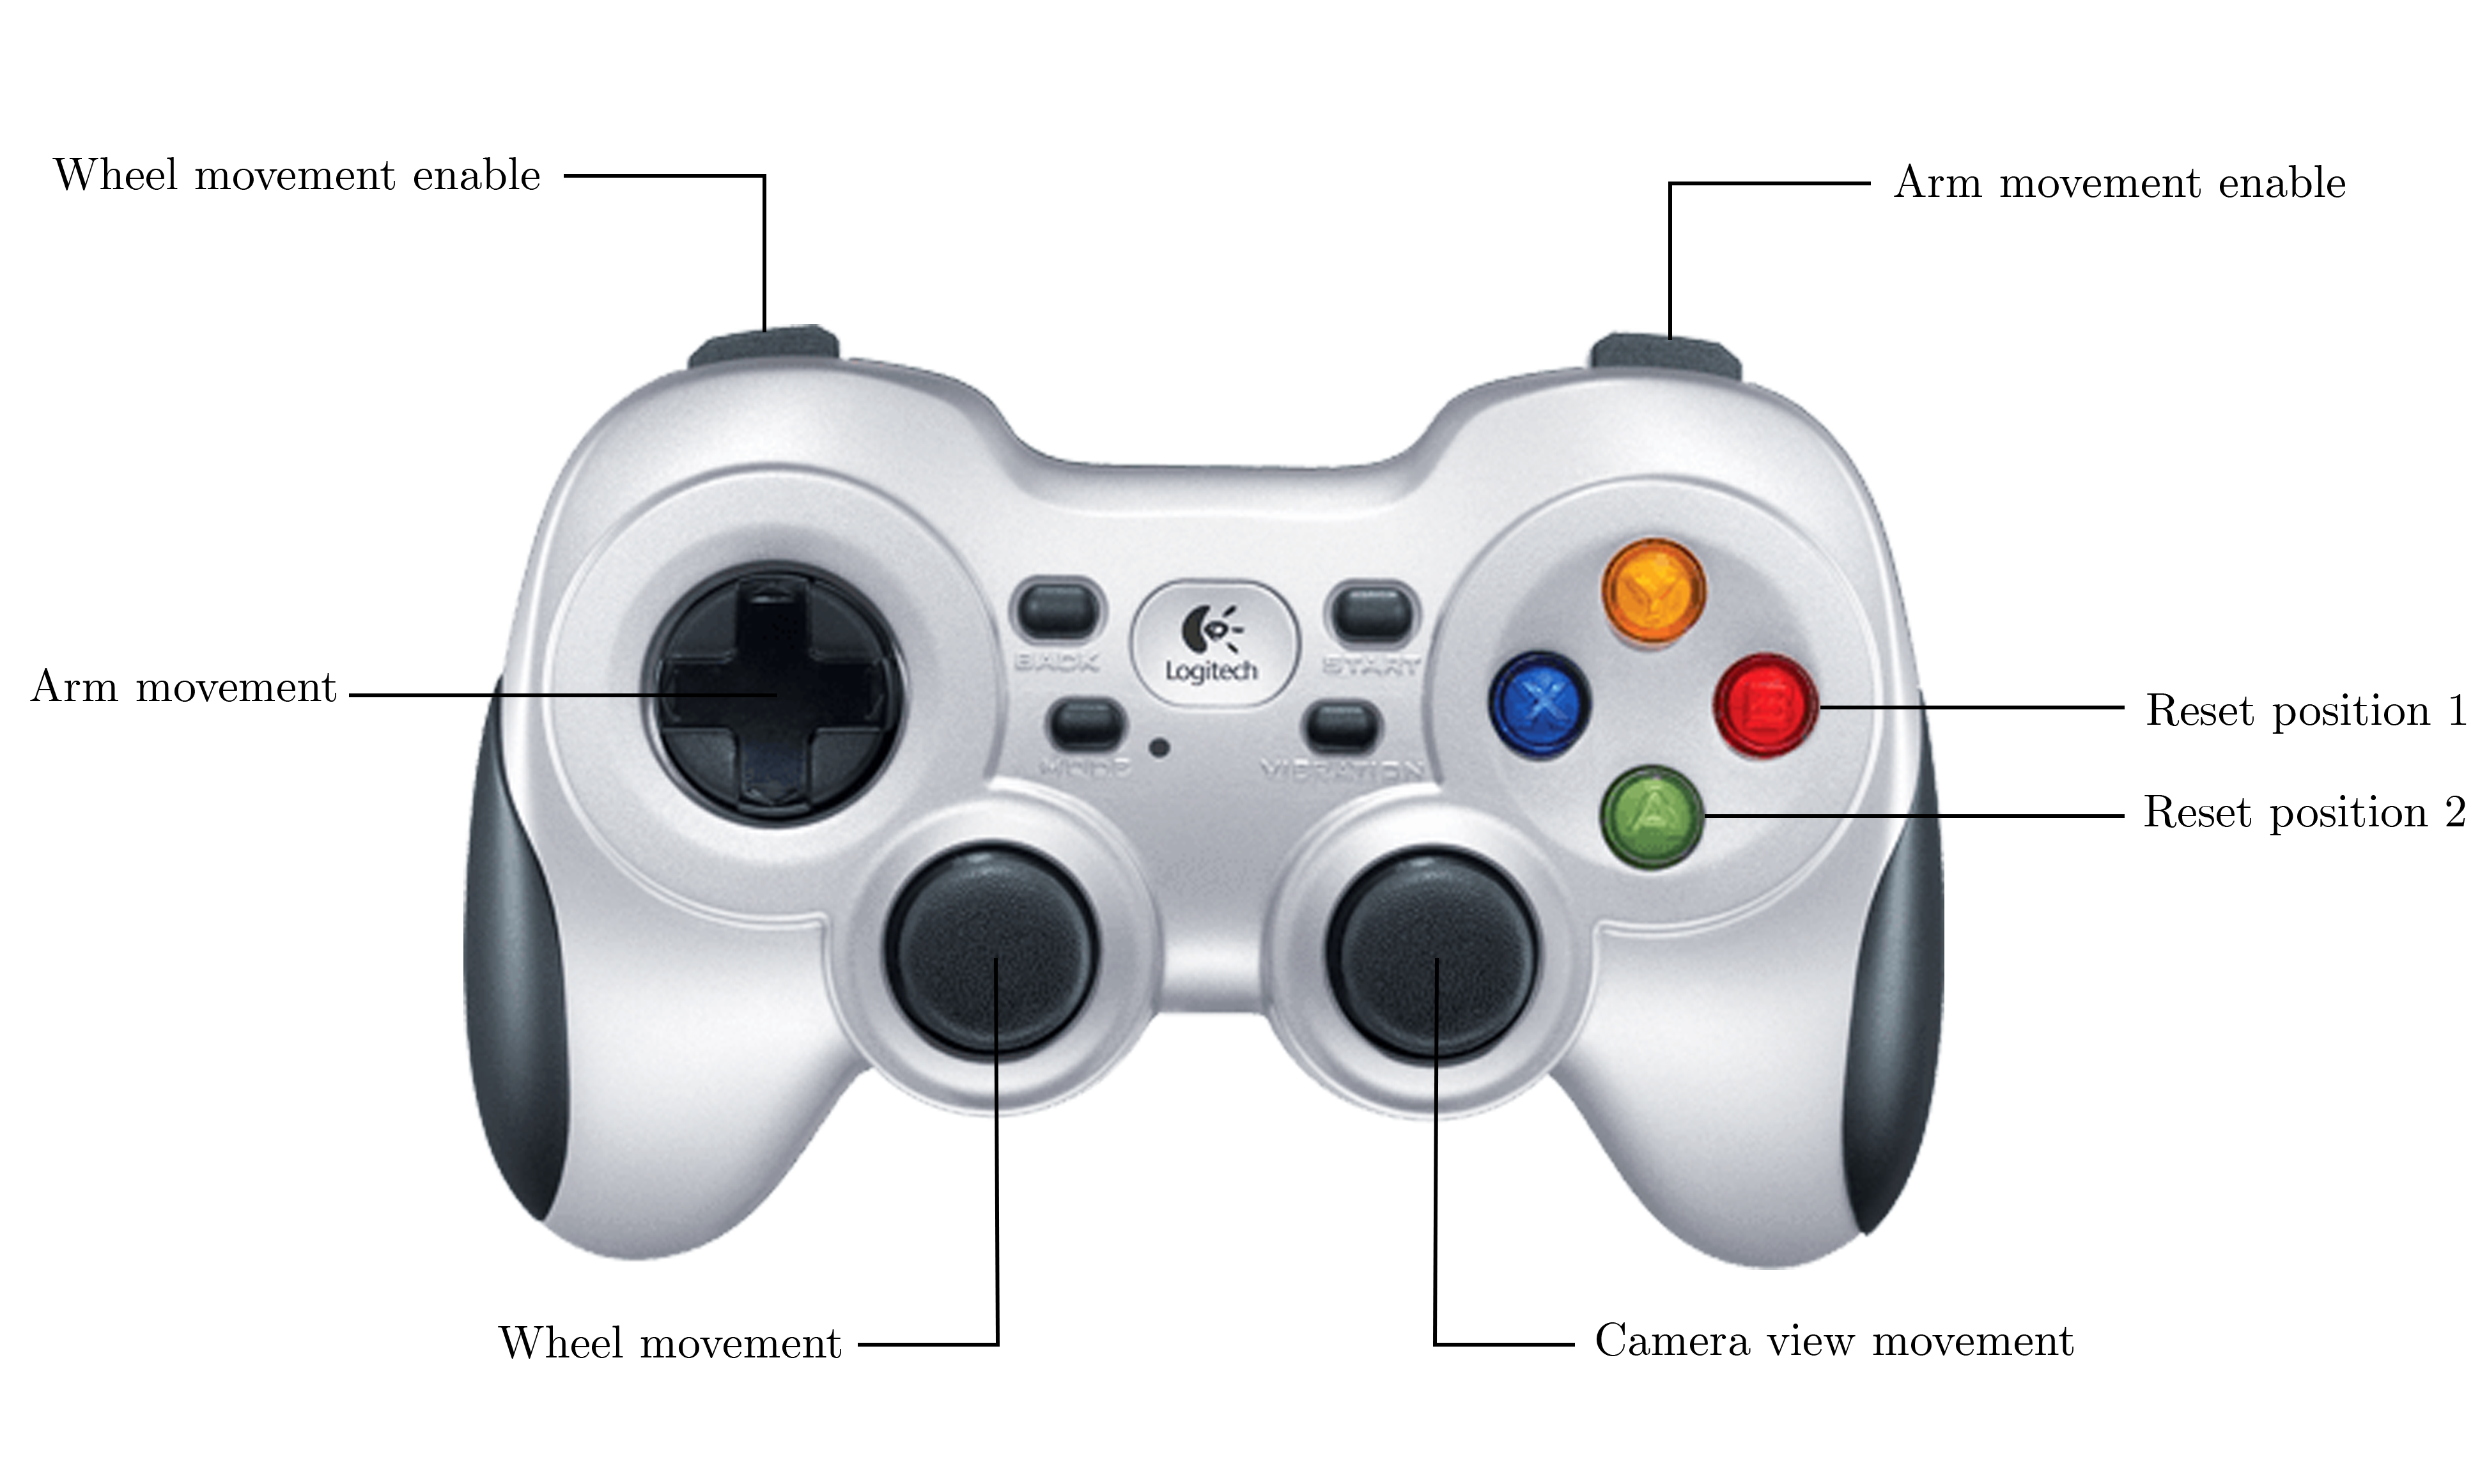
\includegraphics[width=\textwidth]{gamepadedit}
  \caption{Logitech gamepad controller}
  \label{fig:gamepad}
\end{figure}


This node is the interface between the bare joystick drivers and the desired actions. It subscribes to the given topics of type \texttt{sensor\_msgs::Joy} and publishes movement vectors of type \texttt{geometry\_msgs::TwistStamped} to the \texttt{/motor\_command\_vector} and \texttt{/servo\_command\_vector} topics. The gamepad layout used is shown in Figure \ref{fig:gamepad}. \\

\noindent Default reset positions are defined in the launch file and taken from the parameter server at startup. The purpose of these is to provide a fast way to reset the arm and camera position in the case that the robot driver is confused. These are set to the A, B, X, Y buttons on the controller. \\

\noindent The L1 and R1 buttons are used as dead man's switches to to prevent accidental input. L1 is required to be held down for wheel movement, and R1 is needed for camera and arm movement.\\

\newpage
\section{Modelling}
In order for the robot operator to easily visualise the position of the arm, a 3D model is used. The robot and the 3 arm joints are described using a URDF model, with 3 links - \texttt{base\_link} (main chassis), \texttt{arm}, \texttt{head} and \texttt{camera}.\\


\begin{figure}
  \centering
    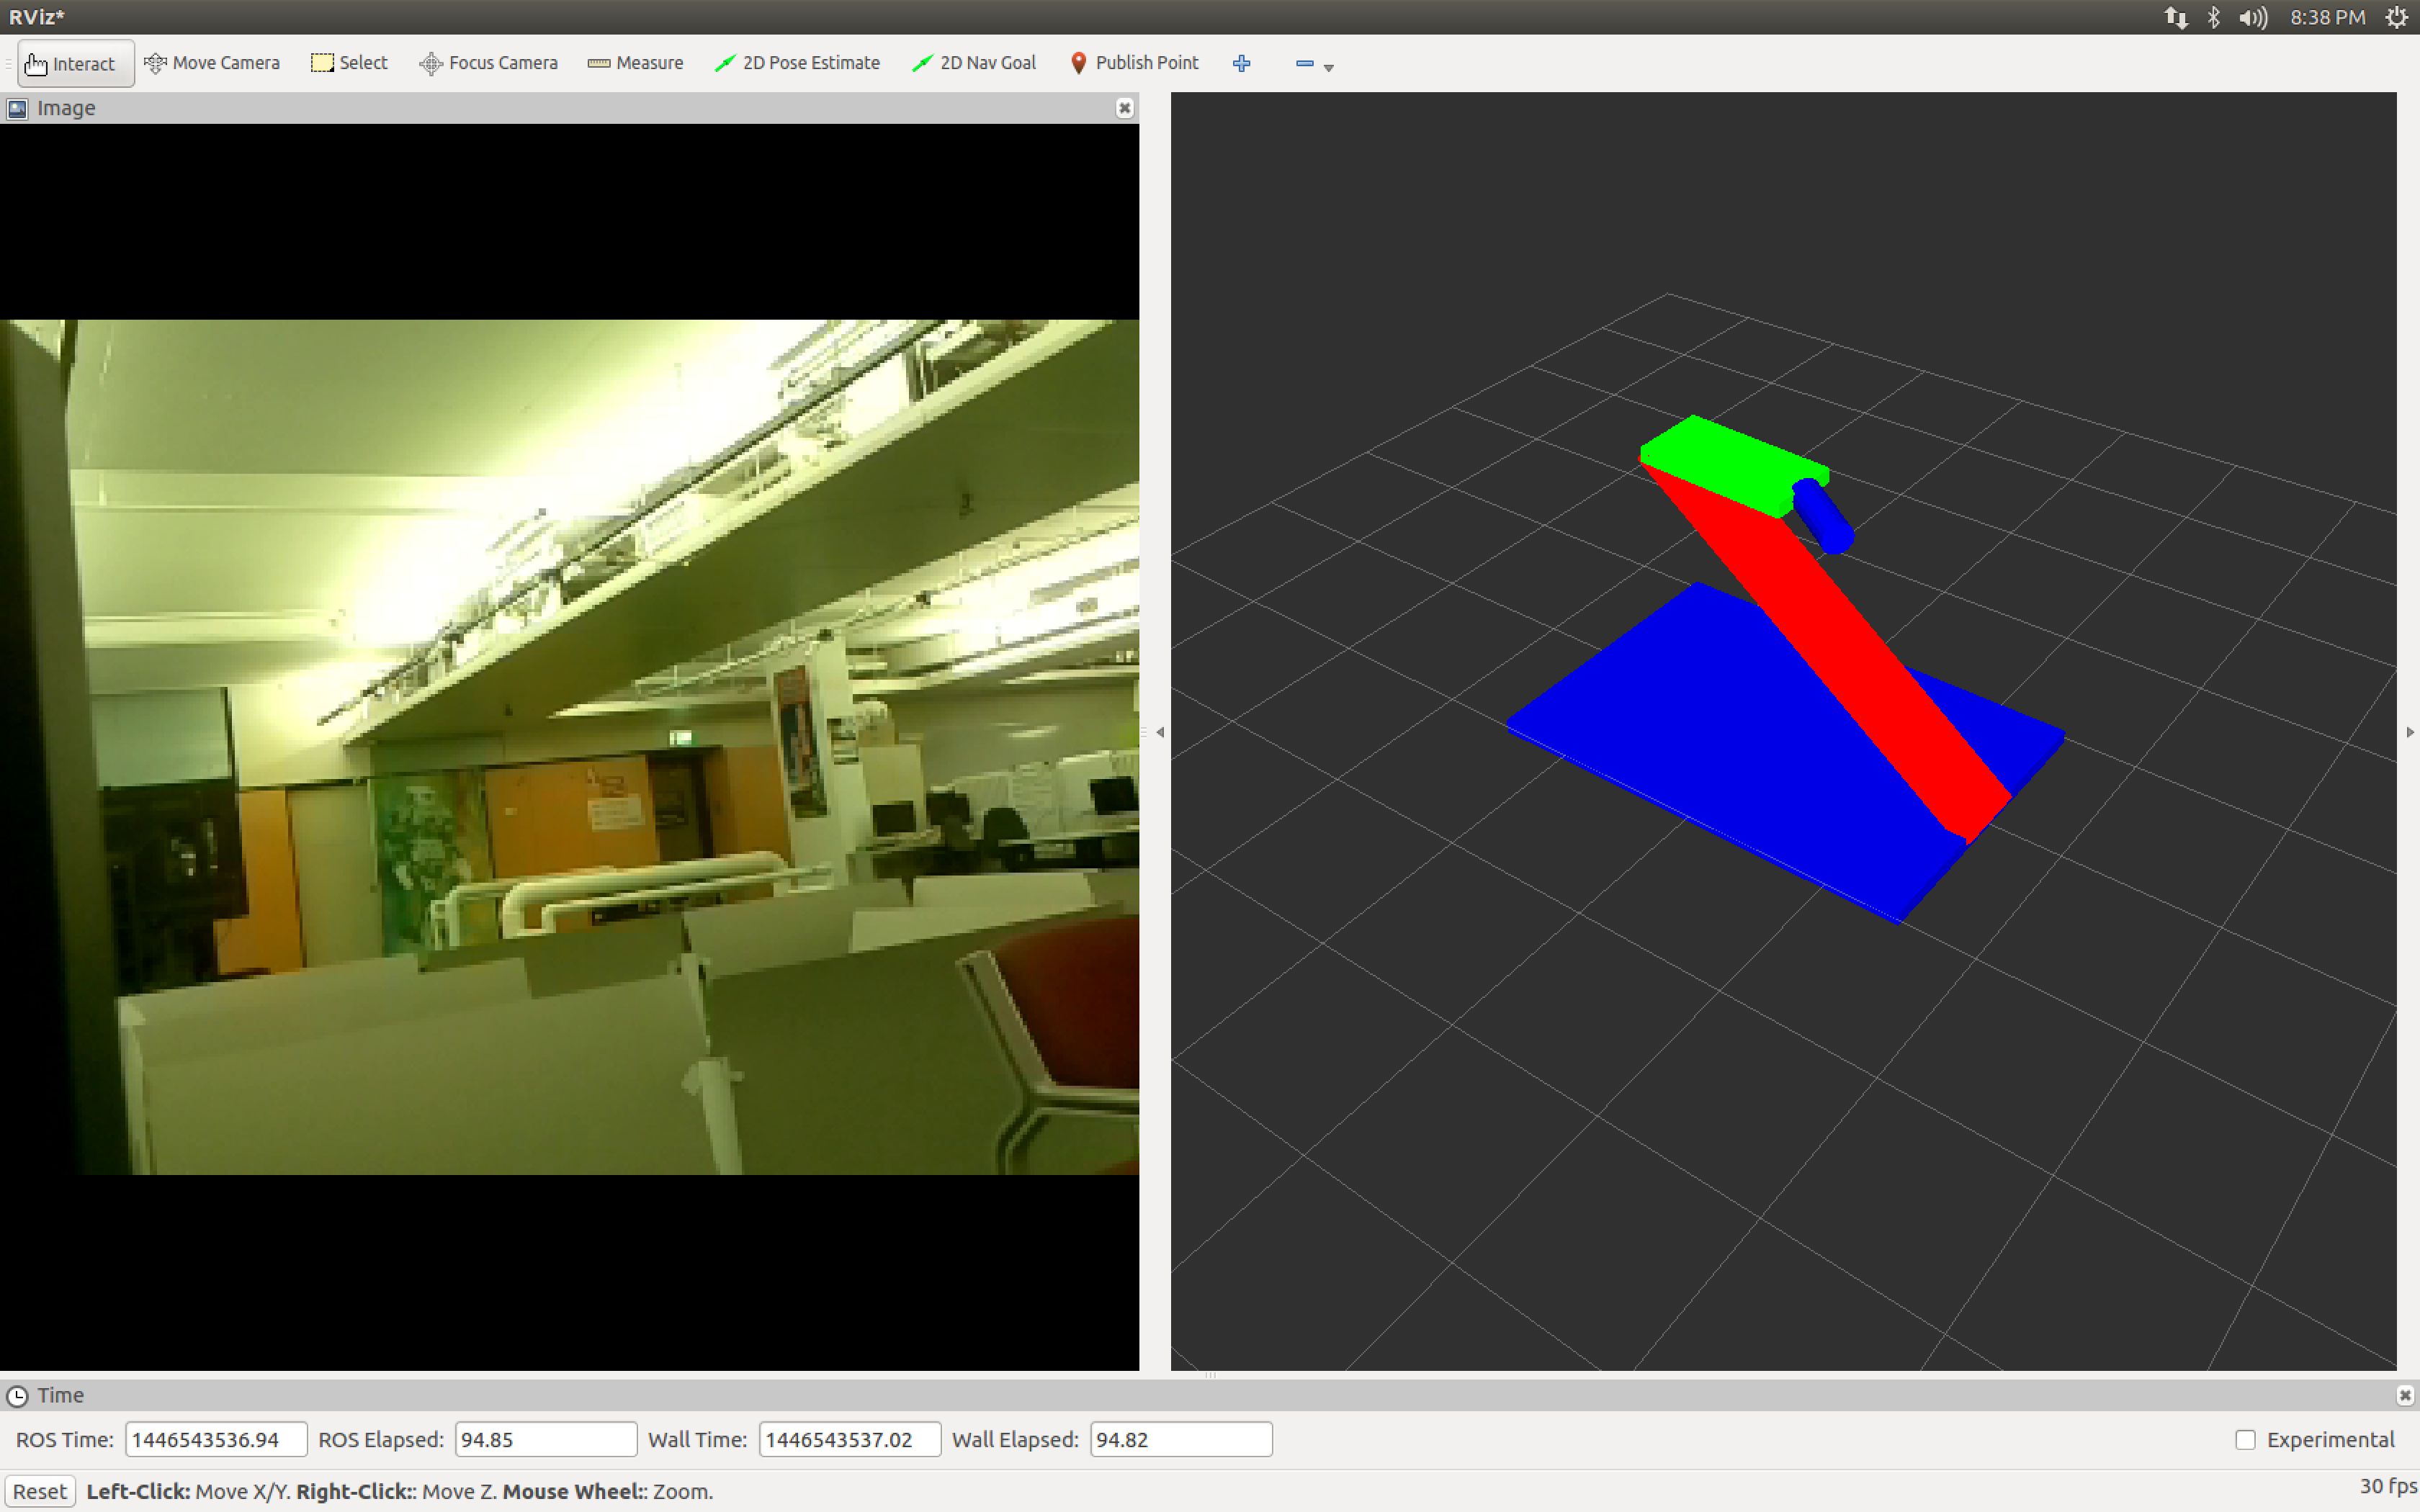
\includegraphics[width=\textwidth]{rviz}
  \caption{Robot operator view}
  \label{fig:rviz}
\end{figure}

\noindent The decision to exaggerate the scale in the model components was done to easily allow the operator to understand the position and angles between joints. Figure \ref{fig:rviz} shows what the operator sees when controlling the robot - the camera stream and the model.

\section{Usage}
On the robot, the \texttt{ass2.launch} file will launch all of the main nodes. In addition, the \texttt{image\_transport republish} node should be launched if compressed image is required. On the operator computer, the \texttt{viewer.launch} file will begin the \texttt{robot\_state\_publisher}, in addition to opening the RViz configuration file, with the camera stream and live 3D model.

\section{Results}
In our project demonstration our Emu's performed well, successfully navigating the rescue course and identifying the victims. The robot operator was capable of controlling the robot using the combination of the camera stream and the robot position model. The narrow angle of the camera, and weight imbalances were the primary difficulties.

\section{Future research}
Possible additions to this project should increase the ease of naviagtion from the perspecive of the external robot viewer. Currently the camera vision is limited by the network bandwith, which requires us to use a small resolution of 640 * 480 and compressed image quality to achieve high frame rates. The use of the 5GHz network in the Runswift lab would significantly improve this.\\

\noindent The addition of a gyroscope to read the angle the robot is tilted would greatly aid the operator in knowing the position and can be easily incorporated into the 3D URDF model to be viewed in RViz.\\

\noindent To aid in the installation process and improve flexibility, an alternative OS could be used such that standard packages are already pre built and do not require long periods of compile time.




\section{References}

\bibliography{testing}
\bibliographystyle{ieeetr}

[1] Robotis, 2010, ‘Robotis e-Manual’, version 1.25.00, Korea [Accessed: 29/10/2015]\\

\noindent [2] ‘ROS Wiki’, ROS/Introduction, (wiki article), May 22, 2014,\\
 Available: http://wiki.ros.org/ROS/Introduction . [Accessed: 02/11/2015]\\

\noindent [3] Salinas, R. 2015. raspicam (version 0.1.3) [software].\\
Available: http://sourceforge.net/projects/raspicam/files/? . [Accessed: 12/10/2015]\\

\noindent [4] Wiki.ros.org, 'dynamixel\_controllers/Tutorials - ROS Wiki', 2015. [Online].\\
Available: http://wiki.ros.org/dynamixel\_controllers/Tutorials. [Accessed: 08- Nov- 2015].\\


\newpage
\begin{appendices}
Appendix A: ROS node graph\\
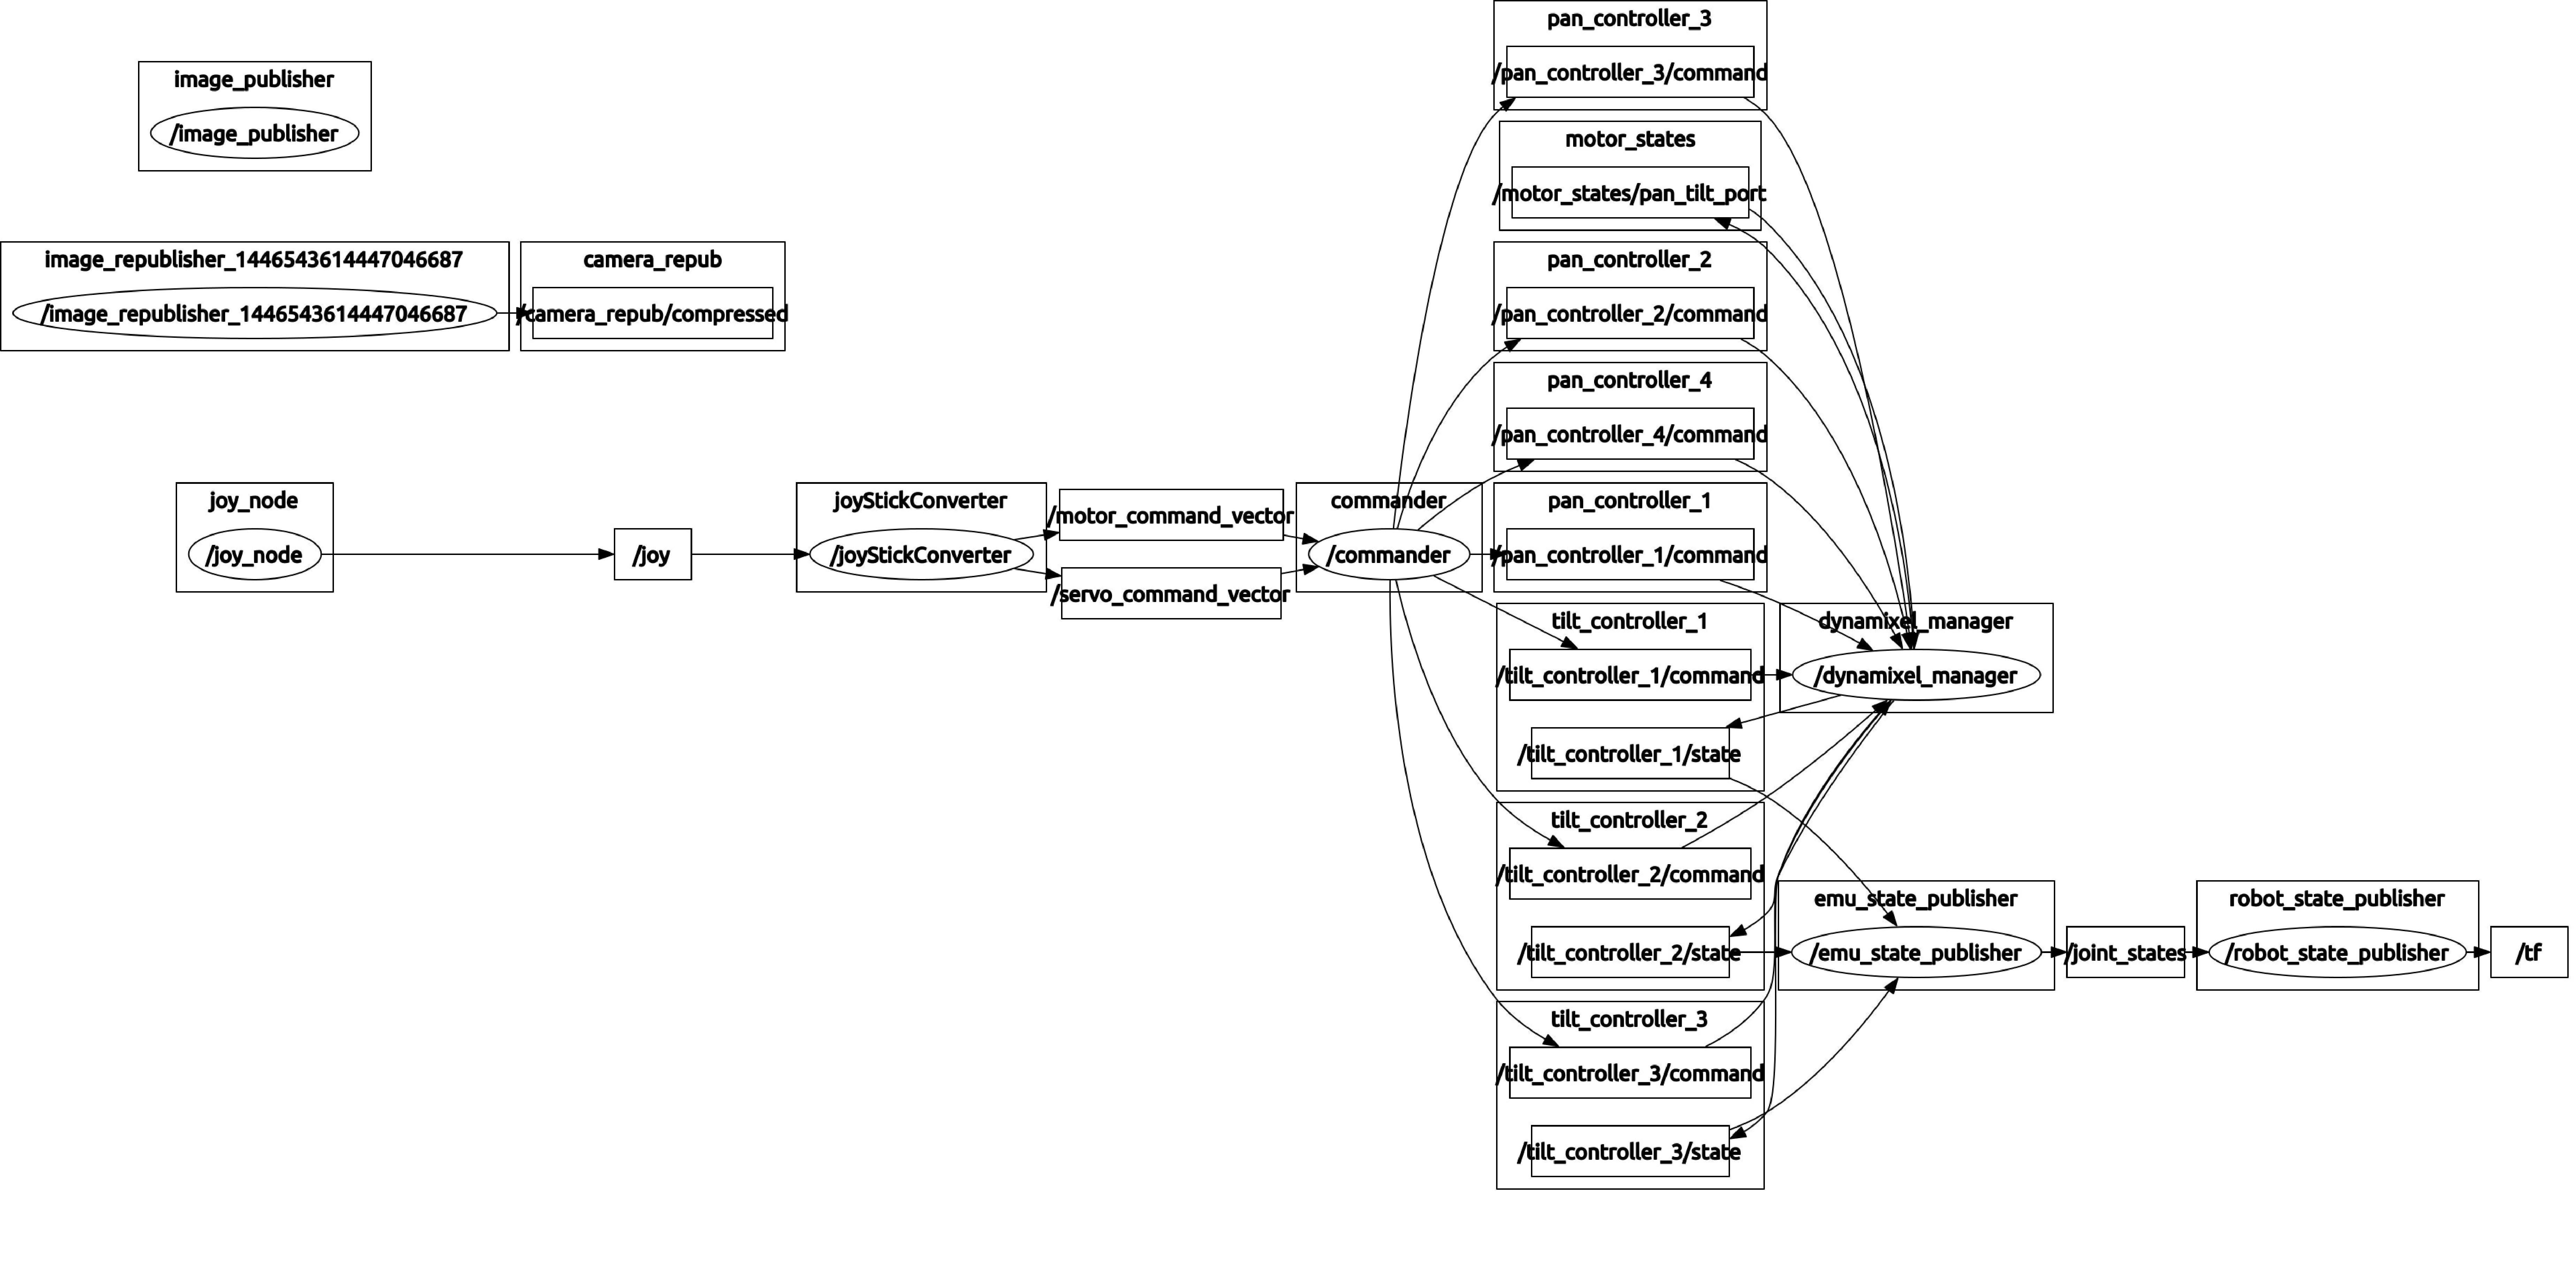
\includegraphics[width=\textheight,angle=90,origin=c]{rosgraph.pdf}

\end{appendices}

\end{document}
